\documentclass[11pt,a4paper]{memoir}
\usepackage{hidde}
\usepackage[pdfauthor={Hidde Boomsma},%
            pdftitle={Dead code elimination for web applications written in dynamic languages},%
            pdftex,
%            colorlinks=true,
            plainpages=false,
            pdfpagelabels
          ] {hyperref}


\newcommand{\AuroraPctAlive}{48.91}
\newcommand{\AuroraPctDead}{51.09}
\newcommand{\AuroraDeadCount}{4973}
\newcommand{\AuroraFileCount}{9755}
\newcommand{\AuroraCount}{1785021849}
\newcommand{\AuroraFirstHit}{2012-04-07 20:56:10}
\newcommand{\AuroraLastHit}{2012-04-09 22:20:25}
\newcommand{\AuroraChangedAt}{2012-03-30 15:18:50}
\newcommand{\MyTwoPctAlive}{35.92}
\newcommand{\MyTwoPctDead}{64.08}
\newcommand{\MyTwoDeadCount}{1552}
\newcommand{\MyTwoFileCount}{2422}
\newcommand{\MyTwoCount}{275159597}
\newcommand{\MyTwoFirstHit}{2012-03-19 16:49:12}
\newcommand{\MyTwoLastHit}{2012-04-09 22:20:30}
\newcommand{\MyTwoChangedAt}{NULL}
\newcommand{\OntrackPctAlive}{68.26}
\newcommand{\OntrackPctDead}{31.74}
\newcommand{\OntrackDeadCount}{293}
\newcommand{\OntrackFileCount}{923}
\newcommand{\OntrackCount}{131381696}
\newcommand{\OntrackFirstHit}{2012-02-16 19:04:06}
\newcommand{\OntrackLastHit}{2012-02-22 13:00:24}
\newcommand{\OntrackChangedAt}{NULL}
\newcommand{\HftTwoPctAlive}{73}
\newcommand{\HftTwoPctDead}{27}
\newcommand{\HftTwoDeadCount}{950}
\newcommand{\HftTwoFileCount}{3518}
\newcommand{\HftTwoCount}{947166185}
\newcommand{\HftTwoFirstHit}{2012-04-07 11:32:05}
\newcommand{\HftTwoLastHit}{2012-04-09 22:20:36}
\newcommand{\HftTwoChangedAt}{NULL}
\newcommand{\HftThreePctAlive}{34.28}
\newcommand{\HftThreePctDead}{65.72}
\newcommand{\HftThreeDeadCount}{1093}
\newcommand{\HftThreeFileCount}{1663}
\newcommand{\HftThreeCount}{565119785}
\newcommand{\HftThreeFirstHit}{2012-03-19 16:23:23}
\newcommand{\HftThreeLastHit}{2012-04-09 22:20:37}
\newcommand{\HftThreeChangedAt}{NULL}
\newcommand{\HftThreestrippedPctAlive}{60.13}
\newcommand{\HftThreestrippedPctDead}{39.87}
\newcommand{\HftThreestrippedDeadCount}{299}
\newcommand{\HftThreestrippedFileCount}{750}
\newcommand{\HftThreestrippedCount}{192806783}
\newcommand{\HftThreestrippedFirstHit}{2012-03-19 16:23:23}
\newcommand{\HftThreestrippedLastHit}{2012-04-09 22:20:37}
\newcommand{\HftThreestrippedChangedAt}{NULL}
\newcommand{\MailbasePctAlive}{45.31}
\newcommand{\MailbasePctDead}{54.69}
\newcommand{\MailbaseDeadCount}{268}
\newcommand{\MailbaseFileCount}{490}
\newcommand{\MailbaseCount}{4856871}
\newcommand{\MailbaseFirstHit}{2012-03-27 16:44:27}
\newcommand{\MailbaseLastHit}{2012-04-09 22:20:27}
\newcommand{\MailbaseChangedAt}{NULL}

\addacronym{svn}{SVN}{Subversion}
\addacronym{vcs}{VCS}{Version Control System}
\addacronym{css}{CSS}{Cascading Style Sheets}
\addacronym{orm}{ORM}{Object-relational mapping}
\addacronym{mvc}{MVC}{Model View Control}
\addacronym{xml}{XML}{Extensible Mark-up Language}
\addacronym{gast}{AST}{Abstract Syntax Tree}
\addacronym{glsurl}{URL}{Uniform Resource Locator}
\addacronym{cgi}{CGI}{Common Gateway Interface}
\addacronym{cli}{CLI}{Command Line Interface}
\addacronym{ide}{IDE}{Integrated Development Environment}
\addacronym{phc}{PHC}{PHP Compiler}
\addacronym{pdt}{PDT}{PHP Development Tools}
\addacronym{dltk}{DLTK}{Dynamic Languages Toolkit}
\addacronym{jit}{JIT}{Just-in-time}
\addacronym{pdo}{PDO}{PHP Data Objects}
\addurl{hostnet}{Hostnet B.V.}{http://www.hostnet.nl}
\addurl{append}{Auto\_append\_file directive in php.ini}{http://php.net/ini.core.php\#ini.auto-append-file}
\addurl{hostnetos}{Hostnet Open Source}{https://github.com/hostnet}
\addurl{zendserver}{Zend Server}{http://www.zend.com/en/products/server}
\addurl{symfony}{Symfony}{http://www.symfony-project.com}
\addurl{d3js}{d3.js}{http://mbostock.github.com/d3}
\addurl{xdebug}{Xdebug}{http://www.xdebu.org}
\addurl{php}{PHP}{http://www.php.net}
\addurl{mysql}{MySQL}{http://www.mysql.com}
\addurl{eclipse}{Eclipse}{http://www.eclipse.org}
\addurl{makefile}{Makefile}{http://www.gnu.org/software/make/manual/make.html}
\addurl{cron}{Cron}{http://linux.die.net/man/5/crontab}
\addurl{bash}{Bash}{http://www.gnu.org/software/bash}
\addurl{epl}{EPL}{http://www.eclipse.org/legal/epl-v10.html}
\addurl{phpcallgraph}{phpCallGraph}{http://phpcallgraph.sourceforge.net}
\addurl{jenkins}{Jenkins}{http://jenkins-ci.org}
\addurl{sqlite}{SQLite}{http://www.sqlite.org}

%---------------------------------------------------------------------%
%                     Options                                         %
%---------------------------------------------------------------------%

\makeglossaries
\title{Dead code elimination for \mbox{web applications} written in \mbox{dynamic languages}}
\subtitle{Master's Thesis \\Version of \today}

% The final version of your thesis should typically use a different
% subtitle without the current date, for example\printglossaries
%\subtitle{Master's Thesis} 
% or remove the subtitle by uncommenting the following line: 
%\subtitle{}

\author{Hidde Boomsma} 
\authoremail{\url{H.B.boomsma@student.tudelft.nl}}
\birthplace{Naarden 1984, the Netherlands}
\studentid{1174371}

% Optional for work done at a company, put this in comments if you did
% not do your thesis work at a company
\company{

\includegraphics[height=1.2cm]{../img/logo-hostnet}\\
Department of Software Engineering\\
Hostnet B.V.\\
Amsterdam, the Netherlands\\
\url{www.hostnet.nl}
}

% Optional (postscript) cover picture. Put this in comments when not needed.
\coverpicture{\center
\includegraphics[width=8cm]{hoster-delft}}


% A copyright notice and maybe something about the cover picture
% Put in comments to get the default copyright notice
\colophon{\noindent
  \copyright{} 2012 \theauthor. All rights reserved \\[1em] 
  Cover picture: Hoster the Hostnet mascot
}

% thesis committee:
\chair{Prof. Dr. A. van Deursen, Faculty EEMCS, TU Delft}
\supervisor{Dr. Phil. H.-G. Gross, Faculty EEMCS, TU Delft}
\committeemember{Dr. S. O. Dulman, Faculty EEMCS, TU Delft}

% The following two are optional for LaTeX (current university
% regulations state that at least one of them should be assigned)
\externalsupervisor{Ir. S. R. Lenselink, Hostnet B.V.}

\setcounter{tocdepth}{2}
\setsecnumdepth{subsection}
\maxsecnumdepth{subsection}

\begin{document}
	\pagenumbering{alph}
	\thispagestyle{empty}
	\maketitle                                      % for the cover page
	\frontmatter
	\makeformaltitlepages{\fontsize{9}{11}
\selectfont
Dead code is source code that is not necessary for the correct execution of an application. Dead code is a result of software ageing. It is a threat for maintainability and therefore should be removed. 

Dead code can be found by collecting the set of code that is used and subtract this set from the set of all code. Collecting the set can be done statically or dynamically. Web applications are often written in dynamic languages. For dynamic languages dynamic analysis suits best and from the maintainability perspective a dynamic analysis is preferred over static analysis because it is able to detect reachable but unused code.

%Via dynamic analysis all unused files are visualized in a tree map in which you can click the boxes to open them like you open directories in an ordinary file explorer. Also an Eclipse plug-in is developed to reduce the impact of existing dead code to the development process before removing it.

In this thesis, we develop and evaluate techniques and tools to support software engineering with dead code identification and elimination for dynamic languages. The language used for evaluation is PHP, one of the most commonly used languages in web development. We demonstrate how and to which extent the techniques and tools proposed can support software developers at Hostnet, a Dutch web hosting organization.

Many organizations in the web domain have the problem that their software grows and demands increasingly more effort to maintain, test, check out and deploy. Old features often remain in the software, because their dependencies are not obvious from the software documentation.

\normalsize}         % for formal title pages with all info
	
	\chapter{Preface}
\label{ch:preface}
This master research is done for \furl{hostnet} from Amsterdam, the Netherlands. Hostnet is a hosting provider active since 1999 and offers domain names in almost all available top level domain names, shared hosting, virtual private and dedicated server hosting. The company has about 165,000 customers and sold approximately 600,000 domain names. Currently Hostnet is the no. 1 seller of the Dutch .nl domains.

Hostnet has it's own software engineering department which takes care of developing all internal systems for the provision of the sold domains and hosing as well as the customer relation management, the web store and web site. All the graphic design is done by the design department. \furl{php} is used to build these complex web applications. Within the company the need rose to delete old program code from the application to make it easier to maintain and upgrade the software, reducing the total cost of ownership. 

I would like to thank the members of the Hostnet software Engineering team for their cooperation and open attitude towards the project and H.-G. Gross for his counselling and pleasant collaboration. Also a word of gratitude for my lovely girlfriend who had to practice a lot of patience when I was working on my thesis and had little time. Last but not least I want to thank my parents for their support and caring.
\vskip1cm
\begin{flushright}
\theauthor\\
Amsterdam, the Netherlands \\
\today\\
\end{flushright}

	\cleardoublepage\tableofcontents
	\cleardoublepage\listoffigures
	\cleardoublepage\mainmatter
	
	\chapter{Introduction}
\label{ch:introduction}

% - What is dead code (in short)
% - Where does it come from (in short)
% - Why is dead code bad
%   o maintainability / human
%   o performance / technical
% - Webapplication
% - Dynamic language

Dead code is source code that is not necessary for the correct execution of an application. Dead code is a result of software ageing\cite{parnas1994,godfrey2000}. Dead code is a threat for maintainability and therefore should be removed. Dead code leads to big applications. Applications with a lot of source are known to suffer from their size when it comes to maintainability and adding new features\cite{godfrey2000,huang2003,kiewkanya2005}. This can be explained because engineers need to understand an application before functionality can be added in the right place. When the programmer is not aware of the dead code, a piece of code that was written years ago and containing unknown bugs could be resurrected. When porting to new versions of used frameworks or libraries effort put in dead code is obviously wasted, therefore it would be beneficial to know which code is dead and remove it.

Besides maintainability dead code has also implications on the performance and resource hunger of an application. If dead code is included in an executable it will cost more disk space and will occupy more memory. Dead instructions can lead to cache misses, lowering performance. Executing useless code also adds up to the total execution time.

Removing dead code requires huge effort\cite{andreopoulos2004,jones2006} therefore a good balance between cost of removal and a perfectly clean source base should be found\cite{scanniello2011}. Making the identification and elimination process more efficient enables us to deliver cleaner code in the same time and give a higher return on investment.

Many organizations in the web domain have the problem that their software grows and demands increasingly more effort to maintain, test, fetch from the \vcs and deploy. Old features often remain in the software, because their dependencies are not obvious from the software documentation.

More and more applications are written for web using domain specific scripting languages such as PHP. As these applications grow more complex the need for quality assurance and software maintenance tools increases. Web applications are in constant motion and are deployed rather than distributed as is the case with regular applications, this makes them very volatile and dynamic. Many web applications make use of dynamic languages such as PHP. These languages are easy to learn and well suited for rapid development of initial ideas. 

A web application differs from a conventional application in the way it is deployed and how the user interact with the application. A conventional program is installed on the users computer and ran on that hardware where a web application is deployed to the company servers and the users connect to it via the web browser. Everything in a web application is done via requests to the server. Each request is handled by a separate thread or process which is terminated or reused after an answer to the request has been send to the browser. It is important to keep the execution time of every request very short because the user will be waiting for the server. When implementing dynamic measuring this should be taken into account. Because a web application request is fairly isolated code that was wrongly removed will not crash the whole system but only show an error page to the user, then the user can push the back button, report the problem and continue working. This is different from conventional applications where all work could be lost when the application crashes. This implies that there is no very big penalty when optimistically removing code that is thought to be dead.

Dead code elimination got a lot of attention regarding performance optimization, but not that much with respect to software maintenance. Techniques used usually perform static analysis to detect code that could not possible be executed. It often concerns optimizations at a compiler level. These optimizations are not applied to the source code and thus do not increase maintainability. There also exist methods to detect dead methods and functions\cite{bacon1996,srivastava1992} which could improve maintainability. Removing dead functions from a dynamic language with static analysis however is very difficult because of dynamic features like run-time source inclusion, dynamic and weak typing, "duck-typed" objects, implicit object and array creation, run-time aliasing, reflection and closures\cite{biggar2009,biggar2009draft,biggar2010,devries2007,tratt2009}.

While static analysis is quite difficult, dynamic analysis is not very hard, because the dynamic nature of the language can be used to conduct measurements without altering the code in many cases. For a static language, static analysis would provide certainty, but in a dynamic environment this is no longer the case. Dynamic analysis, however, will never result in 100\% certainty, but it allows the detection of functionality that exists but is not used any more. From a maintainability perspective this is useful information because maintaining unused code is a waste of effort. Therefore we will use dynamic analysis of the applications at hand to detect dead code. There are two types of dynamic analyses possible, coverage and frequency analysis\cite{ball1999}. The first only captures if a statement, function, method or class is used at all and the second would also measure how often it is used. We have to decide which information will be useful to determine if a piece of code is dead.

The examples used in this thesis are based on the work performed in the case studies at Hostnet.  Hostnet is a Dutch web hosting company with its own software engineering department responsible for the internal infrastructure which enables provisioning, offers customer relations management, the web shop, the customer portal and website. Because Hostnet uses PHP for most of its applications, PHP is used for code examples in this thesis.

%The core business of Hostnet is providing web space and because a lot of people within the company had experience with web development the internal applications are written as web applications in PHP. The customer portal and web shop are obviously also web systems that use the same techniques and databases as the internal applications.


\subsection*{Problem statement and research questions\label{sec:problem}}
The problem of increasing maintenance cost because of the growth and ageing of the software leads to the problem statement.
How to identify and eliminate dead code in dynamic languages in general, and PHP as such language, in particular.

We identified the following research questions in this context:

\begin{itemize}
  \item 
  \textbf{Which data from the software is necessary in         order to perform dead code identification and removal?}  

  Which granularity is needed to provide useful information to the user? Do we need frequency or just coverage information? In short Which information is needed.  This fundamental question is discussed in chapter~\ref{ch:identification} on \nameref{ch:identification}.
  
  \item 
	\textbf{How can we extract the necessary data from the software?}  
  	How is it possible to obtain the required information from the web application? 

	The actual implementation of the system, answering this question on how to fetch the information is presented in chapter~\ref{ch:implementation} (\nameref{ch:implementation}).
  
  
  \item
   \textbf{How should the data be presented to the software developers?} In which way should the date be shown? Should we use graphs, tables or other representations? Could the representation be integrated with the \ide the software developers use?
  \item
  	\textbf{What is the overhead incurred of dynamically extracting the data from the software?}
  	The overhead of the measurement should be small enough to be unnoticed by the end-user of the systems. What is the impact of the overhead and how does it influence the system and server load. The overhead measured in the system will be evaluated in chapter~\ref{ch:evaluation} (\nameref{ch:evaluation}).
  \item 
  	\textbf{What is a good strategy for deciding which code to remove?}
  How long should we wait before we assume that a piece of code will not be ran in the future and can be safely removed? This will be discussed in chapter~\ref{ch:elimination} on \nameref{ch:elimination}.
\end{itemize}

\subsection*{Contributions}
% Method for reducing maintenance cost via dead code removal for web systems
% Quallity assurance in scripted websystems
% Toolset
% Elcipse Plugin

This thesis contributes not only to the body of knowledge about dead code identification and elimination from web systems programmed in dynamic languages but it shows that the proposed method is feasible for use in a business environment. This has been shown via multiple use cases for applications that are heavily in use at Hostnet. A method without to detect which classes are in use without altering the code is devised. The method can handle a constantly changing application as is often the case for web applications. 

To test the method a set of tools has been developed. A plugin for the Eclipse \ide, a web application that can be used to visualize the data and a \cli toolbox that uses the same library as the web application and is capable of collecting and transforming usage data.

These software packages are made open source at github\furl*{hostnetos} under the Hostnet profile.
	\chapter{Dead code identification}
\label{ch:identification}

% - dynamic
% - Still need for static analysis
% - PHP append
% - get_included_files
% - get_executed_functions
% - svn information
% - limitations
% - toolset
% - visualisations

This chapter will explain the different types of dead code and discuss where dead code comes from. In the introduction was already established that dead code leads to a bigger code base which presents an issue for maintenance of the software and therefore should be avoided or removed. After the terminology is clarified the chapter will focus on the granularity of the identified dead code needed to achieve the goal of easier to maintain software. Next the different analysis methods and their implications will be discussed.

\section{Dead code}
\label{sec:dead}

\begin{figure}
	\center
	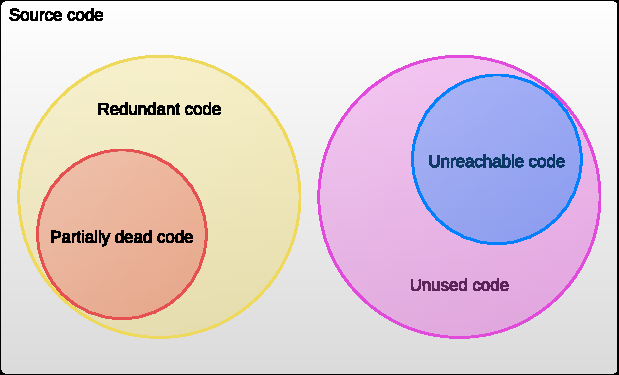
\includegraphics{DeadCodeVenn}
	\caption{\label{fig:deadvenn}Dead code classification, in this thesis dead code is refers to unreachable and unused code}
\end{figure}

The following terminology for dead code is used in literature. 
Knoop\cite{knoop1994} refers to code that is unnecessarily executed when speaking of dead code. Chen\cite{chen1998} calls all code that is not executed on any program path dead code. Janota\cite{janota2007} calls this code unreachable code and code that is unnecessarily executed, redundant code, both subclasses of dead code. Knoop\cite{knoop1994} writes about partial dead code, which is code that is only dead on some program path. 

If looking at dead code we can classify the following sets of dead code: The set of redundant code, code that is executed but does not change the outcome of the program. Partial dead code is a subset of redundant code because it is executed on some paths. Next we have code that is never executed. In this thesis we call this unused code. Some unused code could be executed but never was because the user never used a function to trigger execution of the unused part of the code. Unreachable code would be a subset of unused code. For unreachable code we use the definition of Janota\cite{janota2007}, code that is never executed on any program path. This classification can be seen in \autoref{fig:deadvenn}.

When the term dead code is used in this thesis it refers to unused code, including unreachable code because this is the code we are interested in from a maintenance point of view. From a performance perspective this would not be a problem as long as the source files are not included in the final distribution as is often the case for static languages because the compiler can optimize them out. Redundant code is not included because it can not be determined with dynamic analysis. When we need to be specific the terms partial dead code, redundant code, unused code and unreachable code will be used.

\section{Causes of dead code}

Dead code is not written on purpose, but still almost all applications possess dead code. The following items cause the existence of dead code: 
\begin{description}

\item [Unclear or incomplete specifications] 
Unclear specifications lead to dead code when parts of code are only ran when certain conditions are met. If those conditions are never met in practice because such a case will never arise, those pieces of code are written for nothing due to unclear or incomplete specification. 

\item [Software ageing]
Programming and design mistakes are always made, also in the initial writing of a program. But most arise when changing the software to add new functionality or repair bugs. Changing a program and adding new features will often lead to decay of the structure of an application\cite{parnas1994}. Which in turn will lead to more dead code because programmers are always weary about removing code when they do not have a clear view of the whole program. Dead code because of unused features is a common pattern when software ages. The engineers do not know that certain features are abandoned or simply do not dare remove them\cite{parnas1994,scanniello2011}. When it is known that features are not used any more removing them is not a trivial matter because other parts of the application may have common code with the unused feature. A deep knowledge about the application is required to do so.

\item [Code reuse]
Reuse or reuseability of the software also introduces dead code into an application because not all interfaces and functions will be used\cite{liu1999,tempero2008}.

\item [Modelling objects]
With the introduction of the Object-Oriented programming paradigm it is more likely to model an object and introduce unused methods than with pure procedural code which is only written on demand\cite{srivastava1992}.
\end{description}

\section{Necessary data for dead code identification}

% - granularity
% - collecting information
% - information storage
The first thing to know is what should be measured and to which extent, should statements, methods, classes, components, files or something different be used as smallest unit of dead code, in other words, what will the granularity of the dead code that will be recorded be. The lower the granularity the more information we have available to determine which code is dead. A lower granularity leads to finding more dead code, but also implies more overhead and more data to progress. The overhead should be kept to a minimum and preferable no code should be changed to do the measuring. It is questionable to which extend maintainability can be improved when removing very small pieces of code. Because eliminating dead code needs a lot of effort\cite{andreopoulos2004,jones2006} it is beneficial to start with a large granularity and make it smaller only when there is enough room for improvement left because otherwise too much effort is spend at too little gain. The granularity of dead code identification is a trade-off between overhead and more specific information. We chose the file as smallest unit of dead code to identify. This is part of a top-down approach, first remove dead code at file level and if there is still room for improvement without too much overhead or effort use a smaller unit of dead code, for example a function to get more detailed information.

Because it is impossible to measure dynamically which classes are not used, we measure which classes are used and then take the difference with the set of all classes available in the application. This implies that we can determine which files are dead only after all used files are known. This mean we have to wait until all files that are still in use are expected to be executed. Following conventions used in most languages classes relate to files. Thus if it would be possible to measure included files this would also provide the sought data. The minimum of data that is needed to be able to draw conclusion according a class being alive is coverage\cite{ball1999} data. However to measure how the number of classes in use develops we need more data.  Therefore the first moment in time a class is used should be recorded. It might also be possible that some classes will die within the measurement period. To be able to detect this we also record the last moment in time a class was used. If this date is too far in the past the class can be reckoned dead. Classes that are added to the distribution but still are under development are not likely to be in use and could be mistaken for dead files, it is possible to save the last date a file was changed in the \vcs to solve this problem. To have insight in how many things could be broken when wrongly removing classes from a module, the total number of uses of a class can be saved. This implies a basic form of frequency analysis. This leads to the following list of data to be recorded: number of times used, first time used, last time used, last time edited and changed repository.

\section{Data extraction methods}
% Centralized storage
% Aquire data from multiple sources
% Transform the data
% Aggregate the data
% Modular design
% Adding code to the application
% Registering loaded files or classes
% When to send data to the repository

%dynamic
The data could be acquired by both static and dynamic analysis. But because we look at applications written in dynamic languages and are interested in unused features dynamic analysis is used. 
%The implication of the web application in this context is that all dynamic measurements can be done on a per request base. Because the run-time environment is terminated at the end of each request all used classes (or files) should than be saved.

%aggregate
The data collected should be aggregated directly because storing the raw data would give far too much data to store. Storing raw data could use 1 gibibyte per day for just logging all used files. For example storing 4KiB data $\times$ 4 requests per second $\times$ 3600 seconds per minute $\times$ 24 hours per day = 1.318 GiB per day (Using binary prefixes conforming to \cite{ieee1541}). When measuring applications for multiple months this is simply too expensive. The  4 requests per second is the average that Aurora, the application that will be used for the main use case has during the day. The 4KiB is based on the query size used to update the table in a test set-up for Aurora.

%central
When an application runs on multiple servers or has shared files with other applications the storage should be done on a shared location. All applications send their data to the central repository whereupon the visualizations can be build. 

%recored
There are multiple options to record which files are used by the software. The most generic one is to write a library function which is called from every file upon inclusion of the file. This method can easily be extended to methods, functions and blocks of code. The disadvantage is that adding the function calls can take quite some time if it has to be done by hand. It is possible to the function calls via scripts that automatically add the function calls to the files but it is easy to break things this way. Some scripts may require specific lines to be the first or last in a file which troubles the automatically addition of function calls. When the code base is altered it is very hard to turn everything off and have no overhead any more because all files have to be changed again. An other possibility is to place logging code in the class loading mechanism if the language supports this. This method is preferred over placing function calls in the code because you only have to change the code at one place. The downside is that it is less generic because it can only be used for classes that are dynamically loaded. It is possible to log both classes as well as files that are in use. If the languages uses a garbage collector that can be controlled it is possible to record the elements that were garbage collected. This method has the disadvantage that the objects that are not garbage collected are not added to the set of alive code. If the garbage collector collects all object for the application this could be overcome by calling the garbage collector one last time before exiting the application. The PHP garbage collector can not handle cyclic dependencies\cite{php}, which makes this method not suitable for our use cases.

It is possible that the language at hand offers native support to get a list of all included files, modules or classes. In that case it is possible to use this function and do not worry about all the problems described for the other methods. If a function like this is available this is the preferred method to use. PHP offers this functionality.

%vcs
As described in the section about which data should be available, not only data from the dynamic analysis should be added to the central storage used for the dead code identification but also data from the \vcs should be added. Most \glspl{vcs} can give you the date a file is last edited. This data can be collected and put in the repository as soon as the set of files that will be deployed is known. If possible this should be integrated into the deployment process so that every time that new files are deployed to the production server also new \vcs data is added to the central dead code storage.

%all files
To be able to get from files that are in use by the application to the files that could be dead we need also the set of all files available. This can be achieved by recursively listing the directory contents of the deployed project. In the case of PHP we would only take the \verb|*.php| files into account because we are not interested in non executable files. It is possible to get all available files just before calculating which files are dead but if they are put in the database upfront it is possible to always select which files are used and which are not. This also adds the possibility to create an index of all the files so that the usage information can be processed quickly instead of having to add new files and re-index when more files are used. The performance will stay the same over time when all files are added to the index upfront. Performance will only decrease when more files are added to the application and the index.

%send
Besides collecting all used files, this data also has to be send to the database at some time. Because we are working with web applications the process length is limited to one request form the web browser.   
This leads to the simple decision to send the file names of the used files to the database at the end of each request. This way a minimum number of requests to the database has to be made. 

%Not all languages for the web use the scheme with separated processes per thread. Web applications written in Java and are loaded into memory and handle all requests. For these applications it is possible to select a different moment in to to update the database containing dead code information. For performance reasons it could be beneficial to send the data less often, but sending the data at every request makes sure that if the application crashes there will not be much information lost.

%Foreward reference to visualization
Only recording which code is dead is not enough, the dead code also has to be visualized in a way that is easy for the user to understand and easy to extend when more features or data sets are needed. Therefore the main visualization is build in PHP and javascript as web application. To prevent developers using (possible) dead files by mistake those files should preferably be marked in the \ide{}. More on the visualization can be found in the chapter on visualization (chapter \ref{ch:visualization})

\section{Approach used in this thesis}
For this thesis we use the term dead code for code that is not executed\cite{chen1998}, this includes unused and unreachable\cite{janota2007} code. Redundant code\cite{janota2007} and partial dead code\cite{knoop1994} is not included. Dead code is caused by software ageing\cite{parnas1994,scanniello2011}, code reuse\cite{liu1999,tempero2008}, object modelling\cite{srivastava1992} and unclear specifications. For performance and cost of maintenance\cite{andreopoulos2004,jones2006} the dead files will be identified. If a more fine grained approach is needed this can be done on the files not yet removed. This is left as future work. The data needed to draw conclusions consists of the path of the file, how often it was used and when it was used for the first and last time. \vcs data about when the file was last modified is also added to prevent removing new features that are already in the production system but not activated. The dead files can be detected by recording which files are in use and subtract those from all files. To detect the files in use multiple methods consist. The best one is to rely on a language feature that gives all included files, if this is not possible the class loader or garbage collector could be modified and as last resort calls to a logging function can be added to all files. Because of the amount of data that will be collected everything has to be aggregated right from the start. If the applications are deployed to multiple production servers a centralized storage for the usage data of the files is necessary.

The tools to do this should be very modular so multiple ways of input are possible and the visualizations can easily be reused. The toolbox should allow easy porting to other languages and still be able to use the parts that acquire for example \vcs data.
	\chapter{Implementation of dead code identification}
\label{ch:implementation}

In this chapter the toolbox that is created to be able to perform the case studies is discussed. Before it is possible to look at the implementation directly the differences and properties of the web applications under inspection are looked upon. The visualization of the data can be found in the next chapter (chapter \ref{ch:visualization}).

\section{Web applications in PHP}

The main differences between a web application written in PHP and a conventional application is that the web application is in memory for a very short period and a conventional application resides in memory for the time the users uses it. This means that the application is only active when the user clicks a link or submits data. This could go via a normal HTTP request or through AJAX\cite{garrett2005}. In both cases the browser sends a request to web server which will spawn a PHP process to handle the request and return the result to the browser. When a PHP process crashes, the web page shown to the user will be an 500 error page but the application as a whole will still function. Only just submitted data will be lost, and in most modern browsers pushing the back button will preserve even that data.

Due to the short lived nature of web applications it is possible to just store the aggregated data at the end of every execution. If a page crashes no valuable statistical data will be lost; code that is used by a page that crashes could be interesting to have for debugging purposes but it is of no value for the code in use because the feature clearly does not work. It is worth noting that \furl{zendserver} has functionality to save a full code trace of a crashed page. This could also be done for every page but this will give far too much data to progress because the API does not offer usable aggregation or coverage options. This has to be done afterwards. For a small application this could be possible but for a busy site this will use up the memory.

In a web application the overhead can be measured in the amount of time extra used per page load. The overhead relative to the total length of the page load is not of much importance. Only the time that is extra used for a page is important because if the overhead is too big it will be noticed by the user. For example if a page is very quick and does not have any database interaction the overhead will be really big relative to the total length of execution, but the end user would still not notice this because the load time is still short enough to go unnoticed. This is only true for short lived scripts showing direct output to the user, for a long(er) lived batch job which can be found in the provision system and which are used to create the invoices. For these scripts the overhead relative to the total execution time is important because the periodic tasks could take too long with the dynamic analysis enabled. The goal is to have the overhead go unnoticed by the end users.

\section{Dynamic alive file identification in PHP}
\label{sec:alive}
% - why dead file
% - why this method and not relying on Xdebug or Zend
% - hydrating the database
% - accumulating data
%\image{zend-server}{Zend Server web interface with the auto\_append\_file directive}{fig:zendserver}

PHP offers functionality to retrieve all included files from a running process. To know all files used, this function should be called after the normal execution has finished. Because this function loads all files that are included and does not know if those files are actually used this only provided used files if they are dynamically loaded and are not statically included.  The function call \verb|array get_included_files(void)| gives an array with all files.


Since version 5, PHP has the ability to automatically load classes. This feature is also used by \furl{symfony} the framework used by Hostnet\cite{potencier2010}; it is also used by almost any other framework for PHP. With PHP it is possible to create a function that will be called when a unknown class is instantiated. That function may then take care of loading a file containing the class definition so it will become available before the execution is continued. If the auto load function did not load the needed class definition for the unknown class PHP will fail with an error\cite{php}.

Now we have the method that will give a list of all used files, but those file names still have to be saved in a central database. This has to be done after all normal execution. To accomplish this we could add the call to the \verb|*.php| files that are accessed by the users and web server but PHP offers the possibility to automatically prepend and append files to each and every PHP execution no matter if it is executed through the \cli, \cgi or as Apache module. This property can be set in the  \verb|php.ini|, the global configuration file of PHP, with the  \verb|auto_append_file| directive\furl*{append} This option can also be set via a \verb|.htaccess| file which controls access properties for underlying folders in the Apache web server. This could prove useful to only turn on the analysis for the web server or for some specific directories. At Hostnet we set this property system wide via the \verb|php.ini|. This has the effect that the setting is applied machine wide. So even batch jobs that are started by hand will be taken into account. All logic that sends the used files that have been measured for a request to the central database can be put in to a single file. In this implementation this file is called \verb|append.php| (see \nameref{ch:append.php} for an example implementation). This file is then set to be automatically be appended to every execution of PHP. This files also takes care of the aggregation of the data. The dates in the database about when the file was last used and first used are updated when needed and the usage counter is increased.

MySQL is used as storage solution because it was already available as service at Hostnet and is a very common companion of PHP and Apache. A central MySQL server eases the handling of multiple servers and allows to run all visualization on other server without file transfers. The current implemented solution makes uses of \pdo so the toolbox can easily be integrated with other storage solutions like \furl{sqlite} which does not requires any extra software or drivers to be installed or set-up. This safes the user the trouble of setting up a MySQL server for the sole purpose of analysing one application.

To add files to the database a simple listing is done of the directory structure is used. Only \verb|.php| files are added to the database. When an application is deployed to the production server a new listing is done to be able to remove all deleted files from the database. Files that are not longer in the application will not actually be removed from the databased but only tagged with the date when the removal was detected because with this historic date it is possible to visualize the state of the system in any moment in time since the start of measuring. Every application is primed when a new version of the application is deployed. The deployment of an new application is as simple as an automated \svn checkout on the production server and a new symbolic link to the right folder. After the checkout some (post) configuration is done by the \furl{makefile} in the project. This way other configuration files are loaded for the development, testing, acceptance, staging and production environment are loaded. Via the deployment  Make file the \verb|prime| subcommand of the toolbox (see appendix \ref{sec:prime}) is called.

For every automated deployment system it will suffice to add a call to the \verb|prime| subcommand of the toolbox to the process. If there is no automated process this command should be ran by hand every time new files are added or removed from an application when it is deployed.

As described in the previous \hyperref[ch:identification]{chapter} also \vcs data should be added to the database. This is implemented in the \verb|prime| subcommand that is also used to add the file names to the database as option. Using the \verb|--vcs svn| flag the command will also parse the \svn data of the files. Other \glspl{vcs} can easily be added, most of the work for Git has already been done.

\subsection*{Overview of the implemented tools}
\image{ToolChain}{overview of the dead code identification process}{fig:toolchain}

An overview of the process can be viewed in \autoref{fig:toolchain}. All available files are loaded from disk together with the \vcs data if needed and available. This information is stored in a database and refreshed when a new version of the application is deployed. This database is updated by the \verb|append.php| file adding information about when the file is last used and how many times it is used. The aggregation by \verb|append.php| is done on a file level. From this database containing all raw data it is possible to create graphs showing how the number of used files changes over time, but this data can also be aggregated over the directory structure to provide the percentage of dead code per directory and file. This information can be used for the plug-in. This aggregated data is also used for the tree map visualization, for this visualization the data is cached in an separate database. The tree map visualization also includes the graph. More on these visualizations can be found in the next \hyperref[ch:visualization]{chapter}.
	\chapter{Visualization\label{ch:visualization}}
\label{sec:visualization}

The data that is collected should also be visualized so the user is able to see and use it. The data is collected by the process described in chapter \ref{ch:implementation}. The data collected is stored in a relational database and can also be collected by other methods than the one described in this thesis, this way it is easy to reuse the visualizations. Figure \ref{fig:toolchain} at the end of the previous chapter shows how the visualization is decoupled from the information gathering part that stores all data in the central databases showed at the top of the figure. 

which data should be availabe to the user to be able to make well informed decisions is discussed in the chapter on dead code identification(\autoref{ch:identification}). All this data is visualized in a web application because a web application is multi client and cross platform by nature. Besides the web application there also is an plug-in for the Eclipse \ide. This plug-in displays only the percentage of potential dead files and not all information the web application offers. The Eclipse plug-in is meant to make the developers aware of the possible dead code as soon as possible. Users that do not use Eclipse can always use the web application visualization.


% Tree map
% Eclipse
\section{Tree map}
\image{treemap}{An example of the tree map visualization}{fig:treemap}

The web application uses a tree map \cite{johnson1991} (the red and green boxes shown in \autoref{fig:treemap}) as main visualization method besides a simple sortable table listing the percentage of unused files, the number of unused files, the total number of files and the number of inclusions for the application. The tree map shows the directory structure of the application. The visualization is build up using the directory structure already present on disk to group the files together because this way files that are closely coupled are likely to be in the same (sub) directory, for example modules or plug-ins can be viewed as a whole this way. Because it is easy to spot we have decided to display all files that have been executed green and other files red. Folders get a gradient between green and red depending on the percentage of executed files in the directory. To make it easy to spot which directories only contain executed files or do not contain any executed files these extremes have a distinct green and red color from the gradient start and stop color. The colors and and gradient used is visuble in \autoref{fig:treemap} between the tree map and the table. 

By clicking the boxes in the tree map it is possible to open the clicked directory and view the contents in the same way it was viewed for the parent. This way it is possible to navigate trough the directory structure and view the distribution of dead files over the subdirectories for each directory. As navigational aid a breadcrumb path\cite{hudson2004,lida2003,rogers2003} is shown just above of the tree map. This is the path to the directory that is currently displayed. The directories in the breadcrumb path can be clicked to open them. At the end of the breadcrumb path the directory or file name of the current selected item is displayed. This is convenient to see which directory will be opened when the name is too long to be displayed in the box in the tree map. As short cut the right mouse button opens the parent directory for minimal mouse movement while navigating through the project structure. 

The size of the boxes in the tree map correspondents with the number of dead files contained within the folder to point the user towards the area where the most unused files can be found, the more dead files, the bigger the box will be. A square scale is used so that big folders with many unused files will not take up all space but the difference in size is still distinct enough to be noticed.


When more detailed information is needed it can be fount in the table on the left bottom It possible to sort the list according to each column by clicking on the header. The colors used in the table are the same as those in the tree map. The rows in the table are linked to the boxes of the tree map when hovering the box in the tree map will be highlighted and vice versa. The following columns are available:

\begin{description}
\item[\% $\dagger$] Percentage of unused files in this folder. For a file this is either 0\% or 100\% depending on the state of the file. This number is useful to be able to quickly determine if all files in a folder are not executed until now and probably can be removed.
\item[\# $\dagger$] The number of unused files in this folder. For a file this is either 0 or 1 depending on the state of the file. The more unused files are in a directory the more sense it makes to invest time in this part of the system.
\item[\# .php] The total number of PHP files contained in this folder. For a single file this is always 1. This column can be used to sort the table according to where to project has the most files. This is usable to get a quick overview of the dead code distribution throughout the project and finding caused of dead code like machine generated code that is never used.

\item[\# hits] The number of times this file is included since the beginning of measurement. For folders the numbers of all contained files are aggregated. The number of times files in a directory are included can be used to determine the certainty of the other data displayed, if the files in a directory are only used rarely and over time new files are being included (visible in the first hit column and graph) it is probable that the files that are not used yet will be used in the future, so extra care has to be taken when removing files in such an area of the project. 

\item[age] Date at which the file is last changed. For a folder the most recent date of all contained files is displayed. It is possible that files are just added to the application for a new feature that is not enabled yet. When this is the case the file will be recently changed in the \vcs. If the last changed date in this column is very near the file will probably not be dead even is it is not used yet.

\item[hit time] Date at which this file is included for the first time. For a folder the most recent date of all contained files is displayed. When all files in a folder have very close first hit dates it probably is less probable that the remaining files will be accessed than when all dates are very far apart.

\end{description}

The graph on the bottom right shows the number of unique files used in total over time. The crosses denote the moment when a file was used for the first time. The last data point in the graph is not an actual new inclusion of a file, it is added to plot the graph until the current date (or end of measuring).

These visualizations aid the software engineer when making decisions about when to remove a certain part of the software. It also helps determining where the most benefit could be reached when the goal is to remove all or some portion of the dead code.



This visualization is build using using the \furl{d3js}~javascript~library. This library offers many visualization methods along with the tree map. By using this library it is possible to add other types of visualization of the same data without having to rewrite the whole visualization. The data that is needed for the tree map is provided by a small script that is using the toolbox as library. To view the intermediate format the subcommand \verb|json| of the toolbox can also be run on the command line. 

The data displayed in the tree map is fetched from an hourly updated table in the central database which is build by aggregating the data in the measurement table. This is done via the \verb|tree| subcommand (see appendix \ref{sec:tree}). This command of the toolbox aggregates the number of dead files over the directory structure and stores the number of dead files contained in every directory together with the other fields described above in the description of the table columns.
 
 
\section{Integration into Eclipse}
To aid the developer working with the \ide, there is a plugin to use a (configurable) color scheme like the one in the tree map as colors for the files in the \furl{eclipse} environment. By default the plugin looks for the \verb|colors.txt| file in the project root directory. If it is found all the projects files matching those in the file will be coloured according to the percentage in the file. An example of such a file can be seen in appendix \ref{ch:colors.txt}. The color files for the Hostnet projects are created hourly from the database and saved on a network share accessible by all developers. This way all developers have a fresh view on which files are used in production. The update of the color file happens with the \verb|color| subcommand from the toolbox (see appendix \ref{sec:color}).
\image[\textwidth]{zend-studio}{Eclipse with the dead files color decorator plugin loaded}{fig:eclipse}

	\chapter{Dead code elimination}
\label{ch:elimination}
% user
% vcs
% implications of wrongly deleted files

At this point we have identified code that possibly is dead. We know that used code is not dead, but we do not know whether unused code is not dead.
Before we can declare code dead, we should have an idea about the usage frequency of the code. For example the login page of a system is expected to be used every day, the invoicing system and related files are expected to be used once a month and VAT reports are only used once a year. Knowledge about how much a feature is expected to be used is very important in making the decision if files should be declared dead. 


\section{Decide which code to remove}

When cleaning an application, the first place to start is at the tree map (see figure \ref{fig:treemap}). The tree map shows per directory the number and the percentage of dead files. The size of each box corresponds to the number of dead files in that directory on a square root scale. The square root scale makes sure that directories with little or no dead files are still visible but at the same time spot which directories contain the most potentially dead files. The color of the boxes corresponds to the percentage of dead files contained in the directory. See \autoref{ch:visualization} for a more elaborate description of the tree map.

The tree map can be used to find files clustered together in a folder that are all dead. Files grouped together in a directory are usually related to each other. If a whole folder with related files is dead  it offers a starting point for removal. This method can also be used to detect unused plug-ins if they are located in the directory tree. An example can be seen in figure \ref{fig:aurora_modules}. The modules displayed are those of Aurora, one of the applications that we will look in to with the use case in \autoref{ch:evaluation}. Modules with only dead files can probably be removed if they are not expected to run with an frequency bigger than the period the usage data was collected in. Modules that are only partially dead require more inspection. Here the age of the files can help. If there are two files for almost the same thing and one is dead and the other is not and the dead one is not changed for a long time this could indicate that a feature was updated and the old file was not removed. For this case the graph that shows how many files are executed over time for the directory can be consulted. If the graph is stable for a long period and almost all files are accessed at the same time, it probably is less likely that the other files will be accessed in the future. The number of executions of the files in the folder also indicates the certainty because if it is very low it could very well be that not yet all possibilities and thus files are used.

\image{aurora_modules}{Aurora modules in treemap}{fig:aurora_modules}

The process of selecting code for elimination consists of first searching for the biggest related parts of an application that are marked as possible dead by the dead code identification process. When a coherent possibly dead part is found with no files that were executed we should check wherefore the code is used and if it would be expected to have run. If this is not the case it is possible to remove it. If the feature corresponding to the code at hand is not expected to be executed yet we could either wait for the feature to be used or access it by hand if this has no negative side effects for the operation of the organization. If we have removed all coherent parts of the application only containing dead files we can go on removing files from within these related parts. Here we look at the number of executions for the directory containing the files we want to remove. If this is very low or the graph with the number of executed files over time shows that new files are still executed regularly it is not a good idea to remove files from this directory unless we know that the file should not be used any more and this gets confirmed by the identification process. This process can be viewed in \autoref{fig:process}, the elimination part discussed in the next section is also visible in the figure.

\image{DeadCodeEliminationProcess}{The process of selecting code for elimination and removing it}{fig:process}

\section{Eliminating dead files}
After we have selected code for elimination we can not just remove the code and deploy the application. Before the code will be removed it will go trough a series of steps described in this section. 

When eliminating code the use of a \vcs is of hight importance because this allows to track back which files and methods has been removed and restore them if necessary. A decent process would let the engineer decide which files to remove and put that code change up for review. In this step the files are only removed in the personal system or branch in the \vcs. When the code review is approved, the change set will be committed  
to the current development branch. Now all engineers in the team have the code with the dead files removed. When everything is approved in integration and acceptance testing the change can be used in the next production version (see \autoref{fig:process}).

If code from a dead file is used by other code that code is dead too, otherwise the file would not have been marked dead. Functions that call a class defined in the dead file can also be (partially) removed and so on. The Eclipse \ide with \pdt or Zend Studio can help to find these dependencies, although the \dltk does not offer advanced type inference so it is hard to find all references but it is a start. For now we use full text search of the class and function names. This obviously only works for unique function names. A possible solution for this problem is the identification of dead methods which is described as future work in (\autoref{ch:future}).

When the code is unit tested it is a lot easier to be sure that there are no side effects of removing unreachable code. The code can be removed and if there are no failing tests everything should be fine. The problem lies in removing unused features. Unused features are accompanied by a unit test that also should be removed. 

If continuous integration\cite{fowler2006} is used, it is best to use small commits to the \vcs. This way it is more easy to find which files broke the unit tests. When continuous integration is used defects due to the elimination of files can be detected and handled early. Hostnet uses continuous integration for all projects. 

\section{Effect of wrongly removed code} 

\image{500}{HTTP 500 error page in the webshop}{fig:500}

Despite the effort to only remove code that will never be called upon again it is possible that some used code gets removed. When PHP tries to load a file that is not there it will stop execution with a fatal error and emit a HTTP 500 - Internal Server Error, as shown in \autoref{fig:500}. These error pages are logged by PHP and it is possible to customize an error page so the call stack will be e-mailed to the developers. 

If an engineer receives an email he can remove the part of code calling upon the deleted file or place it back from the source repository. It is worth noting that because it concerns a web application, not the whole application crashes and the user will not lose valuable work because the file was removed. At Hostnet we sent an e-mail report for every internal server error to the developers.

\section{Ceteris paribus not possible}

It is common when taking measurements to only vary one input at a time and keep all other things the same so the effect of that one input can be measured. This is called ceteris paribus, keeping all other things the same. Because the measurements take place in a live application it is not possible to freeze it from updates for at least several months to acquire the right measurements in a undisturbed situation. Especially in the fast moving web world this is impossible. Therefore we have to cope with the fact that there are updates coming in all the time. This implies that unused code is not always dead. It could be that it is just not used yet or that it is just added to the application but not enabled for the end-user yet. To be able to detect this last type it is possible to take \vcs data into account. At Hostnet almost all projects are stored in \svn and some bleeding edge ones in git. Using this data it is possible to detect that a file is recently added to the system and therefore should not be declared dead. The date a file was last change in the \vcs is displayed in the age column shown in \autoref{fig:treemap} as described in \autoref{ch:visualization}. To get a better view on the certainty that new features will be accessed for a directory it is possible to look at the graph (also in \autoref{fig:treemap}) which shows new files accessed over time. If all new files added to an application would also be displayed in this graph it would not give a good view of the certainty because files for newly added feature would be included making it look that it takes longer to stabilize then is the case in reality. By not adding files to the graph that has been added later on this problem is prevented. The files will still be displayed in the tree map for a complete overview of the application.
	% EVALUATION
% Identification
% - Overhead
%   + Which overhead
%   + How is it measured
%   + Is it being noticed
% - How long does it take depending on type of application and how much it is used
%   + comperation of Hostnet applications with graphs
%   + setup of measurement
%   + measurement period
%   + measurement servers
% Elimination
% - Web application visualization (tree map)
%   + is the displayed data usefull
%   + is it usefull in determining which parts to remove
% - Eclipse plugin
%   + does it hinder the developer in daily work
%   + does it prevent mistakes
%   + is it clear what the colors mean to the developers
% Applicability (other organizations)
% Threats to validity





\chapter{Evaluation}
\label{ch:evaluation}

In this chapter we will discuss and evaluate the proposed method for dead code elimination. The evaluation is done by implementing dead code elimination at \furl{hostnet}. Hostnet is a Dutch web hosting company with its own software engineering department of about 10 engineers. The main language used at Hostnet is PHP because many people in the web hosting business are familiar with PHP and use it because it is easy to learn and adopt and facilitates rapid development.

We will evaluate both the data gathering part: dead code identification and the data processing part: dead code elimination. For the identification part we are mainly interested in the overhead of doing runtime analysis and in determining how long the analysis should be performed before we an say with sufficient confidence that code is indeed dead. The overhead is measured in the code identification part that is implemented in Aurora, the biggest application (in number of files) in use within Hostnet. Because the overhead is dependent on the number of files in use in the application should be the worst case within Hostnet. We compare 6 applications developed within Hostnet to see how long it will take until we can tell if the files that are not executed can be regarded as dead files. These application are all different in the way they are used, the number of features and how often they are used.

Both the visualizations and the method for dead code elimination are evaluated. The Eclipse plug-in  is installed for all team members and used by 8 of them currently working on PHP projects. This plug-in is used in the development of all applications done at the moment. The Eclipse plug-in should not hinder the engineers and should we would like to know if it helps the developers by letting them focus on files that are actually used. This is difficult to measure in numbers so we used a questionnaire to evaluate the Eclipse plug-in.

The web application visualization with the tree map is only used by 3 people that really removed code form Aurora. For the evaluation of the proposed process of dead code elimination (see \autoref{ch:elimination}) we tried it on Aurora and managed to remove more then 28\% (2740 files) of the files within just a day work. The evaluation of the visualisation will focus on how the web application is used by the engineers and how they base their decisions on the displayed information (see \autoref{ch:visualization} for a description of the user interface).

For the evaluation of both the visualizations a questionnaire is used. For the evaluation of the dead code elimination process as described in \autoref{ch:elimination}, the evaluation is based on the observations made while the engineers removed the files and monitoring the application to see if there would be any bugs that were caused by the deletion of files. 

The chapter will end with an discussion on the applicability of the method for dead code elimination described in this thesis and the threats to validity of the findings reported in the evaluation.

%Applicability
%Overhead
%Accuracy


\section{Overhead}
\label{sec:overhead}

The overhead caused by reporting all used files to the central database should be low enough to not be noticed by the end user of the application. At the end of each request from the browser for a new page, a list of used files is sent to the central database. Prior to building up the connection and sending the list, the response from the web application is flushed to the browser. This way the browser will already render the web page and only indicates that the page is still loading. This is convenient because even when the overhead is noticeable the end user can still access the application without delay.

We look at the overhead in time per page request. Profiling code has been added to the analysis in Aurora to measure the overhead. Aurora is the most used application within Hostnet and has the biggest number of files. The overhead in Aurora should be the worst case within Hostnet, as the time to send the list to the database and process it, is dependent on the size of the list and the load on the database server. Concurrent write operations to a single MySQL data base on the same row will lock and create bigger load times when the load on the server increases. It is very likely that the same row will be updated in every request to the database because every request to Aurora will pass through the \verb|index.php| file which is the starting point for the application.

When measuring the overhead, the time spent on the analysis is measured as well as the time required to build a connection to the database to be able to see if network congestion could be a limiting factor. A plot of this overhead can be viewed in \autoref{fig:overhead}. On the x-axis the time spent in milliseconds is shown. On the left y-axis the frequency of the corresponding amount of overhead is displayed. In red the overhead for the creation of the connection to the MySQL database on the database server is plotted. The time needed to build the connection has an average at 1.6~ms with and standard deviation of 0.6~ms. The connection overhead seems normally distributed with a standard deviation of under 1~ms and without additional peaks which indicates there is no congestion on the network. In green the frequencies of total overhead have been plotted. The average overhead is 7.8~ms with an standard deviation of 153.5~ms. The blue curve denotes the probability that the overhead will be less than the corresponding value on the x-axis. Here we can see that in over 95\% of the measured cases the overhead stays below 6~ms.

\image[.9\textwidth]{overhead}{Overhead caused by measuring included files (in memory)}{fig:overhead}

When we use a slower method of storage, for example on disk storage in the database server we notice that two peaks will appear in the total overhead curve (see \autoref{fig:overheaddisk}). These appear because if the table is locked the query will have to wait a few milliseconds. Using disk storage, the average overhead is 27.5~ms with an standard deviation of 231~ms. Still in 80\% of the cases the overhead is below 10~ms. In 95\% of the cases the overhead is below 23~ms. The problem of locking rows is clearly visible here. The use of a memory table will not solve this problem but helps us determine where the peaks came from. For the analysis at Hostnet the slower on disk storage is used so that there is no need to build a backup mechanism to make sure that when the database server would be restarted the data would not be lost. 

\image[.9\textwidth]{overhead_disk}{Overhead caused by measuring included files (on disk)}{fig:overheaddisk}

When the load on the database becomes too high other solutions must be found to keep the overhead within bounds so it will not be noticed. One solution could be to use multiple MySQL servers and aggregate the date between them less frequently then the normal updates occur. An other solution could be to aggregate the data on the web server side in shared memory and send it to the server at a frequency less then that of the page requests.

From the experience at Hostnet we can say that the overhead was not noticed by the helpdesk and account managers using Aurora for every day work even when using disk storage. We found that the limiting factor is not the project size but the frequency of requests because locks in the database will occur that create a bigger overhead than the time needed to send the list of files to the database.


\clearpage
\section{Dead Code Identification}

In this section we look at how long we have to wait until we can use the results of the dynamic analysis. Therefore a case study has been done. The overhead measurements in the previous section are gathered from this use case. For about three months 6~Hostnet applications are analysed. The applications differ in age, the number of users that uses them and  the complexity in number of features they possess. In \autoref{tbl:ages} the applications used for the case study are shown. The number of users and features are relative to the other applications. We present the idea that small applications with a lot of unique users will offer certain results faster then a big application with little features. Further we check if the older applications within Hostnet have more dead code than the recently developed ones.

For every application a short introduction about the use of the application in the organization will be given together with a graph that visualizes the number of files used by the application over time. When this graph stabilizes it means that the probability that new files will be included decreases. The graph shows the number of files in the application accessed over time. The last data point in the graph denotes the end of the measurement and not a new file that is included.

All Hostnet applications are build as web applications, written in PHP. All tested applications make use of the \furl{symfony} framework and are connected to a \furl{mysql} Relational Database Cluster. Using Symfony also implies using the auto load functionality the framework offers. This makes all applications suitable for this analysis. The use of MySQL or Symfony is not needed for the implemented identification method to work, only the dynamic loading of files is.

\subsection*{Applications in the use case}
In \autoref{tbl:ages} the 6~applications that will be used in the use case are shown. The applications are developed in the past 6 years and all written in PHP. There are 4~applications, Aurora, My Hostnet, the Web shop and Mailbase that are accessed by humans, the other two, HFT2 and HFT3 are provisioning system that run (mostly) without user interaction. From the 4~web applications Aurora and Mailbase are only for internal use within Hostnet. The Web shop and My Hostnet are accessed by customers. The value of page requests for Aurora in the table has been adjusted to take the number of automated request from some monitoring systems into account. These systems are responsible for almost half of the requests but always request the same page. An example is the TV which shows real-time data about which customers are currently in the web shop.

\begin{table}[b]
	\small
	\centering
	\begin{tabular}{|l|l|l|l|c|r|}
	\hline
	Name & Description & \# files & Age & \# page requests / day\\
	\hline
	HFT3        & New provision system        & \HftThreestrippedFileCount & 1 year  & n.a.    \\
	Web shop    & web shop                    & \OntrackFileCount          & 3 years & 39,643  \\
	Aurora      & CRM application             & \AuroraFileCount           & 5 years & 60,383  \\
	Mailbase    & Lagacy mail filter frontend & \MailbaseFileCount         & 5 years & 2,803   \\
	My Hostnet  & Customer portal             & \MyTwoFileCount            & 5 years & 53,495  \\
	HFT2        & Provisioning system         & \HftTwoFileCount           & 6 years & n.a.    \\
	\hline
	\end{tabular}
	\caption{Applications ordered according to age	\label{tbl:ages}}
\end{table}



%\addtocounter{footnote}{-1}
%\footnotetext{HFT3 included a plugin for the \orm which is available through the Symfony framework for the other applications, this plugin is not taken into account here.}
%\addtocounter{footnote}{1}

\newcommand{\hftTwoFootnote}{HFT2 uses static includes in the legacy part of the application which is not supported. Static included files always report as alive, increasing the percentage of used files significantly. Not all files are included statically so the method is still usable to identify dead code and eliminate it but comparison to the other applications does not make much sense.
}
%\footnotetext{\hftTwoFootnote}



\subsection*{Aurora}
Aurora is the biggest (in files) and most feature rich application developed at Hostnet. It is used to store all customer information. Everything from contact information, bought products, contracts and invoices. Aurora takes care of a lot of the periodic tasks like creating invoices\cite{boomsma2008}. Aurora also offers all kind of statistics and development tools for the Software Engineering department. Aurora is used for daily business by the majority of employees, most work consists of looking up customer data, like contracts, contact data and products. All the advanced function are only used once in a while.

The server has to take care of about 4 visits per second on average. This is because all helpdesk employees use Aurora for almost all their tasks and some TVs which show real-time statistics via Aurora.

Aurora is build up in clearly distinctive modules, batch jobs, database models, plug-ins and templates.
When looking at the. All modules that are not changed recently are probably dead. Before removing a module it is needed to know what it is used for and if it was already expected to be used or not. If it was not expected to be used it can be removed. This shows that selecting files for removal requires human reasoning.

\bottomimage[1\textwidth]{usecase/aurora_saturation}{Number of used files over time in Aurora}{fig:aurora_saturation}

When looking at the graph for the application in \autoref{fig:aurora_saturation} we can see it rises quickly and then keeps growing steadily, the slope of the graph never reaches 0. At the end of January an increase in the number of files is visible, here a new version is deployed and a cache rebuild took place. The cache rebuild used a lot of new files in the database model of Aurora. That the graph is increasing unit now means that new features are still being accessed every day even after 3 month time. For Aurora as a whole it is very likely that new files will be used in the future, however sub modules may be stable in less time. 

Because in Aurora as a whole new files are being accessed every day, it is not possible to draw a general conclusion for the whole application other than that it is not yet possible to start with dead file removal other than for clearly separated parts like modules that only contain dead files or core functionality which is frequently since the start of the analysis.

The first moment when the data becomes useful is at the point the slope decreases substantially and the graph bends. In the graph of Aurora this point is visible at the 14th of January. From this point all base functionality has been accessed. Aurora has a lot of monthly jobs, so we should at leas wait a full month until we start using the data. After this time we can start with the dead code removal. The graph should not shows sudden increases in the number of used files any more at this time, if it does there might be something wrong with the estimation of the frequency wherein features are used.

If we would look at the graph and make an educated guess about the asymptote it will approach of about 5000 just to be on the safe side, we could calculate the probability of deleting a file that will be used in the future (when randomly choosing one). 9755 total files - 5000 alive files = 4755 dead files. 4983 files are not used yet. 4984 unused files - 4755 dead files = 229 alive files not accessed yet. 229 dead files not accessed yet / 4983 files not used yet = 0.046. This gives a change of 4.6\% that a file would be removed that was not dead when random selecting a file. These numbers are not included in the visualization because they are based on a educated guess of where the asymptote would be. Building a model to predict the probability of removing alive files at a given point in time is left as future work.

\subsection*{My Hostnet}

My Hostnet is the customer portal of Hostnet. When somebody owns a domain name, virtual private server or hosting they can login to My Hostnet to view their address data, invoices, products and so on. It is also possible to change settings for products, upgrade products, pay invoicess or cancel contracts.
\\
\hereimage[1\textwidth]{usecase/my2_saturation}{Number of used files over time in My Hostnet}{fig:my2_saturation}


My Hostnet has a lot more different users than Aurora and far less features. The graph in \autoref{fig:my2_saturation} shows a quick rise over just several days and then the slope is 0 for more than a month, then a couple of new files is included because a very rarely used feature has been accessed (in this case an error page that was resurrected for use in a new feature). Although new files may always be used in the future, the dead file identification in My Hostnet stabilizes after about 7~days. Then it is reasonable safe to remove the dead files according to the described dead code elimination procedure. We can conclude that we can start measuring after 14 days. All features of My Hostnet are expected to be used at least once a week. With the exception for error pages. The 7~days needed to stabilize is taken form the graph based on the fact that no new files were accessed afterwards for several months. When using the same method as for Aurora to calculate the probability as we did for Aurora the probability of removing an alive file when random selecting one approaches 0.


\subsection*{Web shop}

The web shop has a high number of page requests and a relatively low number of files (see \autoref{tbl:ages}, although the web shop is highly dynamic and can generate different versions of the web shop based on where the customer came from. Because not all features of the web shop will be activated at all times and there are some very specific feature for rarely sold products, it is to be expected that the web shop will stabilize faster than Aurora but slower than My Hostnet.

When looking at the graph in \autoref{fig:ontrack_saturation} we see that after 30 days still some new files where used. But we can also see is increasingly more time between new files being included. We can also see that the graph became stable after half February. Around 20 February the slope of the graph already was 0 but this was only for a few days. The distance between the point should be bigger than the expected frequency of the features of the application. For the web shop we know that some products are sold only once per month. It is possible, however, to start dead code elimination at this point as long as we keep in mind that all files related to products, especially the ones sold less often, could still be needed.
\hereimage[1\textwidth]{usecase/ontrack_saturation}{Number of used files over time in the web shop}{fig:ontrack_saturation}

When looking into the measurements concerning the web shop we can see that a lot of code that is identified as dead code actually belongs to deactivated features in the order module. When new features will be activated they will only show up in the graph if the files were already deployed on the production server at the time the files were first indexed. Once again we see that dead code identification on the scale of files needs human reasoning. Here we can also see that when an increase is seen in the graph it may be worth investigating where it came from, because if it was caused by enabling a feature we can still consider the graph stable. In the future automatic notification of such events could be implemented.

\subsection*{HFT2}
HFT stands for Hostnet Full Throttle and is the provisioning system used to order all domains and deliver them to the customers, the HFT2 also sets up hosting accounts and mails all needed information to the owner. There are a lot of products that can be delivered through the HFT2. 

The HFT2 is the oldest application under inspection and is not yet (and never will be) fully converted into a Symfony application. This explains the low percentage of dead files; the unconverted part of the HFT2 uses static inclusion of the needed resources. This marks all included files as alive, not telling if they are actually in use.


\hereimage[1\textwidth]{usecase/hft2_saturation}{Number of used files over time in HFT2}{fig:hft2_saturation}

As a consequence, the applied method only works well on the Symfony part (116 dead files). This, by no means, render the method useless for the other part. Because the application is fairly aged a lot of old files that are never included can be found in the legacy part (935 dead files). The plots also show that not all inclusions are static in the old part of the application because new files are included over time.

When we look at the graph in \autoref{fig:hft2_saturation} we can see that the slope approaches zero around 28th of January but that still some new files are accessed later on. These files are visible as the crosses in the line. The last cross only denotes the end of the analysis. However if we would look at the Symfony part of the application we can see that no new files were included within a month. The files that were included in the old part of the application later on, are some specific products and the logout feature in the interface. This shows that we have to be carefull when removing code that is related to products that are not regularly sold. The logout function that is used after some time shows that some features are seldom used. For seldom used features it is questionable if we should keep them. It is arguable that a feature that is only accessed once in the three months should be removed because it costs more time than performing the task by hand.

From the employees of Hostnet we know that a part of the HFT2 is transformed into Symfony and a old legacy part is still there. In the visualization the legacy part of the application might be recognizable by the fact that most of the files have not changes for 6 years. The fact that there is a folder called Symfony in which all files are more recently added would confirm this.

\subsection*{HFT3}
HFT3 is the successor of HFT2 and uses a new database model which is put in a shared repository. At this time HFT3 is the major application using the new database model but in the future more applications will be using it. Action should be taken log and accumulate data for shared code in a separate dataset which is used by all applications which make use of that code to see which code is in use. Libraries could also be analysed in the same way. At this moment we have to hard code different locations to store usage data in the dynamic analysis. It could be possible to automatically generate the location bases on  \vcs data in the future.

HFT3 is a lot smaller (in files) that HFT2 but it is used just as much. The work rounds in which HFT3 fetches data and execute it's tasks are  a lot shorter than in the previous version. 

Allmost all dead files can be tracked down to the database. 807 dead files are located in an \orm plug-in. This plug-in is not included in the other projects because it is bundled with symfony, but the HFT3 uses a newer version so it is included. The percentage of dead files when not taking this plug-in into account drops from  65\% to 40\%. This percentage is more in line with the measured values in the other applications and shows that newer applications probably have less dead code.

\hereimage[1\textwidth]{usecase/hft3_saturation}{Number of used files over time in HFT3}{fig:hft3_saturation}
When we look at the graph for the HFT3 in \autoref{fig:hft3_saturation} we can see that over time new files are still being accessed. When we look further into the HFT we can see that some of the new files belong to an \orm plug-in (which should be outside of the project). The only new file accessed that does not belong to the \orm plug-in contains an Exception class which was used after one month. This leads to the conclusion that the HFT3 has to be measured for about one month to get sufficient certainty.

\subsection*{Mailbase}

Mailbase is is used to view and search all email that is send to and received from customers as well as  mail to domain registrars. Only the user interface is under inspection. Mailbase is almost never used. The code is written using the Symfony framework and is the smallest (in number of files) of the tested applications. 

\hereimage[1\textwidth]{usecase/mailbase_saturation}{Number of used files over time in Mailbase}{fig:mailbase_saturation}

Because Mailbase is used very little it is hard to know when new features will stop showing up. In the graph in \autoref{fig:mailbase_saturation} we can see that the distance between new files being included does not lengthen yet, so there is no indication to assume the graph is stabilizing. This means we can not use the data for maintenance purposes as we can for the other applications.

At Hostnet only one person is still using Mailbase. Everything that he does not use will be removed from Mailbase and the functionality that remains will be ported to Aurora. In this case the only way to get accurate data is to ask the one person sill using the application. An option is to just port only the functionality used in the past 3 month and add all other functionality only on request with the old Mailbase code in the \vcs as reference. This shows that depending on the goal it is possible to use the dead code identification method even when an application is used by only one user.


\subsection*{Results of the case study}

Now we got data for all applications we can compare them and see if the applications behave as we thought within Hostnet. First we look at the age of the applications. We expected older applications to have a lower percentage of used code than the more recent ones. 

If we order the applications according to their age, and we compare that with the ranking according ranking according to the percentage of unused files, then we observe that

 \autoref{tbl:used}. In \autoref{fig:all_apps} the graphs that were used to determine when to start with dead code elimination for every application in the use case are combined into one figure. In this figure the x-axis still denotes the time but it is given in days instead of dates, because not all use cases were started at the same time and thus they would start at different dates making it harder to compare them. This is also the reason for the fact that not all lines in the graph end at the same position. The y-axis uses a percentage instead of the number of files so it is possible to compare the applications in this graph according to percentage of used code. This figure shows that, in general, no conclusion can be drawn on how long you have to wait before starting dead code elimination.
 
When looking at \autoref{tbl:used} we see that the HFT2 does contain less unused code than the other applications even though it is the oldest one. This is because a big part of the HFT2 is statically included and denoted alive even if it would not be used at all. The HFT2 also has a newer part of the application which uses dynamic inclusion. This part shown as the HFT2 (Symfony) entry in the table. We also notice that the HFT3 uses less of its code then the web shop does despite of it being younger. This can be explained the fact HFT3 contains relatively much shared and generated code. The shared code can be found in the model of the HFT3 which also contains classes for a new mass mailer system.
 
In general we can say that older applications tend to have more dead code within Hostnet. We also see that code reuse is an important source of dead code in the Hostnet applications. Dead code is found in plug-ins for all application.

The second prediction, that small applications and much used application  will reach a stable analysis faster than little used complex ones. We look at \autoref{tbl:time} to see if this is the case for the applications at Hostnet. The division of the number of files by the number of page views per day is taken to compare it to the time needed to stabilize we found in de case study. We see that the prediction is only partly confirmed. The web shop took longer than was to be expected based solely on the number of features and users. We see that it is important to know what type of features an application posses. For example in the web shop some rarely sold products are available that require extra information from the client. The files needed for those products are expected to be only used once a month. This demonstrates that a rough estimation can be made on the number of files and users but that for a better estimation it is needed to know when the application features are expected to be used. We can also see that for Hostnet the time we had to wait to be certain ranges from 1 week to (at least) over 3 month. It is possible to already eliminate dead code from stable parts of the system. In the use case on dead code elimination (next section) we successfully removed dead files from Aurora where new files are accessed every day.

\begin{table}[p]
	\small
	\centering
	\begin{tabular}{|l|l|l|l|l|c|c|}
	\hline
	Name & Description & Age & \% used\\
	\hline
	HFT3    		         & New provision system         & 1 year  & \HftThreestrippedPctAlive\% \\
	Web shop             & web shop                     & 3 years & \OntrackPctAlive\%          \\
	HFT2 (Symfony)       & Provisioning system          & 3 years & 50.64\%                     \\
	Aurora               & CRM application              & 5 years & \AuroraPctAlive\%           \\
	Mailbase             & Lagacy mail filter frontend  & 5 years & \MailbasePctAlive\%         \\
	My Hostnet           & Customer portal              & 5 years & \MyTwoPctAlive\%            \\
	HFT2\footnotemark    & Provisioning system          & 6 years & \HftTwoPctAlive\%           \\
	\hline
	\end{tabular}
	\caption{Applications ordered according to age with percentage of used files\label{tbl:used}}
\end{table}

\begin{table}[p]
	\small
	\centering
	\begin{tabular}{|l|r|r|r|l|}
	\hline	 
	 Name        & page views $/$ day & \# files & $\text{\# files}/\text{\# page views}$  & no new files accessed after\\
	\hline
	My Hostnet & 53,495 & \MyTwoFileCount            &  0.045 & 1 week\\
	HFT3       & n.a.   & \HftThreestrippedFileCount &   n.a. & 1 month\\
	Web shop   & 39,643 & \OntrackFileCount          &  0.023 & 1 month\\
	HFT2       & n.a.   & \HftTwoFileCount           &   n.a. & 2 months\\
	Aurora     & 60,383 & \AuroraFileCount           & 0.161 & Not yet\\
	Mailbase   &  2,803 & \MailbaseFileCount         & 0.171 & uncertain\\
	\hline 
	\end{tabular}
	\caption{Time to wait before now new files are accessed any more per application\label{tbl:time}}
\end{table}
\footnotetext{\hftTwoFootnote}

\pageimage{usecase/all}{Ratio of used files per application}{fig:all_apps}


% Elimination
% - Web application visualization (tree map)
%   + is the displayed data usefull
%   + is it usefull in determining which parts to remove
% - Eclipse plugin
%   + does it hinder the developer in daily work
%   + does it prevent mistakes
%   + is it clear what the colors mean to the developers

\section{Dead code elimination}



In this section the dead code elimination process using the created visualization tools is evaluated. The process and tree map visualization is used by two people for a full day to test the described process (\autoref{ch:elimination}) and remove dead parts of Aurora. The Eclipse plug-in is installed for all team members and has been used for a full month by the time of writing. Both visualizations and the process are evaluated using a questionnaire, because it is extremely difficult to measure objectively how the visualizations aids the developers eliminating dead code. The Eclipse plug-in could already reduce some of the maintenance cost of dead code without actually removing it by preventing the developers to mistakenly search for a bug or search for a functionality in a file that is not used.

For the visualization containing the tree map, table an graph of used files we look at how the various components of the interface are used and if the user finds them useful. This is done in the questionnaire with the questions that can be seen in \autoref{tbl:treemap}.

\begin{table}
\begin{tabular}{p{7cm}ccccc}
%\toprule
\textbf{Question:} 
& \rotatebox{90}{fully agree}
  \rotatebox{90}{very useful}
& \rotatebox{90}{agree}
  \rotatebox{90}{useful}
& \rotatebox{90}{disagree}
  \rotatebox{90}{useless}
& \rotatebox{90}{completely disagree}
  \rotatebox{90}{completely useless}
& \rotatebox{90}{do not know}
\\

\cmidrule(r){1-1} \cmidrule(lr){2-2} \cmidrule(lr){3-3}\cmidrule(lr){4-4}\cmidrule(lr){5-5}\cmidrule(lr){6-6} 

The tree map helps me to find dead code:                                         & 3 &   &   &   & \\
I know where I am in the project structure when browsing the directory structure & 1 & 1 & 1 &   & \\
I use the graph in my decisions about code removal                               & 1 & 2 &   &   & \\
I use the table when looking for dead code                                       & 2 & 1 &   &   & \\
Rate the usefulness of the following entries in the table                        &   &   &   &   & \\
\hspace{2em} path                     &3& & & &\\
\hspace{2em} percentage of dead files & &3& & &\\
\hspace{2em} number of dead files     &1&1&1& &\\
\hspace{2em} number of .php files     &1&1&1& &\\
\hspace{2em} number of hits           &1&1&1& &\\
\hspace{2em} age                      &3& & & &\\
\hspace{2em} hit time                 &1&2& & &\\
%\bottomrule
\end{tabular}

\caption{Questions about the tree map visualization\label{tbl:treemap}}
\end{table}

As is visible in \autoref{tbl:treemap}, the questionnaire was only taken by 3 people because it was not possible to spare more people for a day of dead code elimination. Two of them worked one full day on removing dead code from Aurora using the tree map visualization. When we look at the answers we can see that the tree map points users in the right direction to find the unused files that can be removed and that it is found helpful. The same is true for the table and the graph. When looking at the columns in the table we can see that data that is already available in the tree map is rated less useful then data that is available only in the table. Also the total number of PHP files seems of less interest than the other data. Nobody rated a part of the interface completely useless. Maybe the interface should be improved to make it more visible which project and directory is currently viewed because this was not clear to all participants. Although it is not possible to draw general conclusions from such a small data set, it is possible to say that the visualization did help the engineers to locate, select end eliminate dead code. 

We managed to reduce the size of Aurora by 28\% in less then a day's work with two people. So far, no defects were found related to the  removal of that dead code.

The Eclipse plug-in was also evaluated using the same questionnaire. For the Eclipse plug-in 8 people gave their opinion on how they use and like the plug-in. The participants consist of three senior developers, five junior developers. The questions and aggregated answers are in \autoref{tbl:eclipse}.


\begin{table}
\begin{tabular}{p{9cm}ccccc}
%\toprule
\textbf{Question:} 
& \rotatebox{90}{fully agree}
& \rotatebox{90}{agree}
& \rotatebox{90}{disagree}
& \rotatebox{90}{completely disagree}
& \rotatebox{90}{do not know}
\\

\cmidrule(r){1-1} \cmidrule(lr){2-2} \cmidrule(lr){3-3}\cmidrule(lr){4-4}\cmidrule(lr){5-5}\cmidrule(lr){6-6} 

I have the dead files plug-in enabled all the time            & 5 & 3 &   &   & \\
I turn the plug-in only on for the purpose of removing files  &   &   & 4 & 4 & \\
The plug-in aids me when debugging applications               & 4 & 2 & 2 &   & \\
The plug-in aids me when developing new features              &   & 5 & 3 &   & \\
A file that is red can be removed                             &   & 1 & 4 & 3 & \\
A fully green folder only contains live .php data             & 4 & 4 &   &   & \\    

%\bottomrule
\end{tabular}
\caption{Questions about the Eclipse plug-in\label{tbl:eclipse}}
\end{table}
When we look at the answers (see \autoref{tbl:eclipse}), we observe that people have the plug-in turned on all the time and do not turn it off despite the fact that they were shown how that would be done. This leads to the conclusion that the plug-in does not get in the way of the developers. Next we want to know if the plug-in also aids the developers with their everyday work and if they understand what de colors mean. Most people find it especially useful when debugging, some others also when developing new features. When looking at the raw data it is possible to see that everybody found the plug-in useful for at least debugging or developing new features. The last to questions were added to test whether the participants knew what the colors precisely mean. A file that is red is not used in production, but on only that fact is not enough to justify removal. A fully green folder does indeed only contain used .php files, although it is possible that it will contain other unused resources. We can conclude that in general people do know what the colors mean and find them useful in their everyday work. I got a lot of positive feedback about the plug-in from the team at Hostnet.

\section{Discussion}
In this section the findings and short coming of the presented method for dead code identification and elimination will be discussed based on the case study results. Also applicability and threads to validity will be looked upon.

The implemented method should be enhanced to be able to measure a shared code base, this will not be much trouble. To also take statically included classes into account more work research should be performed if this is possible with an PHP plugin or that modifying the source is needed.

Outside PHP the method is applicable to all languages which use an auto loading mechanism to dynamically load classes and allow modification of this mechanism or an other method to list all loaded classes. This means the method is applicable for Java, but not for C and C++ programs.

The overhead observed is about 8~ms on average for the fast in memory storage and about 27~ms on average when using disk storage. Overhead only appears at the end of every page, all content is already send to the client, only the connection is not closed yet because this would end the execution of the PHP script, which results in a slightly longer visible load indicator in the browser but all information will be available to the user without delay.

The use cases provided useful data on how to measure an application. They also showed that how long you have to wait before you get useful data is dependent on how many actions are performed on the system and how these actions are distributed along the features and the number of features. For the web shop, customer portal and provisioning system it is not needed to wait longer than 2 month.

When looking at the tested applications measured we observe that an older application usually has a higher percentage dead code within Hostnet. This also is to be expected because more code remains as a program ages. This can be seen in figure \ref{fig:all_apps} and in table: \ref{tbl:used}. This property can not just be generalized, because it depends a lot on how much effort is put in keeping the application small by the development team\cite{scanniello2011}, but within Hostnet everything is build by the same team which makes it possible to compare the applications.

When removing code, searching for code referring to dead code is a tedious job, but the color decorator plug-in in Eclipse aids with this, because not only the files, but also the search results are decorated. This means that when the programmer searches for method invocations of method in a dead file all files containing those invocations will also be coloured in the search result. Automatically indicating the methods that call methods in dead files should be the next step to easy the programmers job.

\subsection*{Applicability}
% dynamic loaded files
% administrate loaded files

The discussed method for identifying dead files can be used in environments where files are dynamically loaded at run time. As long as files are only loaded when there actually used it is possible to add tracing code to the application or use language features to get a list of all used files. The method will not work in environments where files are statically loaded at run time or are compiled in to an executable.

In practice this method will not work for compiled languages like C and C++ because there will be no files any more when the the application is compiled into an executable. For languages that dynamically loads files like Java does for classes 

The tree map visualization and the Eclipse plug-in can be connected to any data source about dead files. For example determining which images or other resources are used in an web application can be done by parsing the web server access log files and fed into the central database. The visualization tools created will now be able to show information for images without customization.

The procedure for dead code elimination is based on the fact that the analysis is dynamic. It should be equally valid for removing other resources or code with a different granularity as long as the data is dynamically gathered.

The tool box created for the case studies can be reused without modification in every PHP application that uses the auto load functionality instead of statically including all files.

\subsection*{Threads to validity}
% - Application with low number of users
% - Applications with static files
% - Developers ... ?? difficult to foresee.
% - Comparing applications is not possible (??)

There are some important threads to validity of the results. The method will only perform well for applications which are used very much. It is not possible to get accurate data from an application only used a few times a weak by a couple of users. A second thread is that the application should not make use of static file inclusion, this would not make the data less reliable but certainly less usable because all static included files will be marked as alive. The use of already available code coverage tools could be used to circumvent this problem in situations where an overhead of several times the normal execution time is no problem.

The toolbox and method are especially developed for use within Hostnet. The method has not been tested on applications outside of Hostnet.

When a comparison will be made between different applications it is important to only measure those files that are maintained by the team the measurement is done for because otherwise unused features of plug-ins or a framework will pollute the statistics.

Elimination of dead files sill is a humans job, this implies that somebody with better knowledge of the code will likely be more efficient in removing the dead code than somebody that is not familiar with the application at hand. This could compromise a clear view on how well this method performs and how the tools aid the developer. Somebody that knows the application well can be more accurate for some parts than is possible then when only using the data from the visualizations.

The current overhead data is only valid for a MySQL database. It could be worse when using an alternative way of storage for the central database. This said, MySQL is freely available to everybody and could be used when needed.

The usefulness of the visualization and the elimination of dead code is only evaluated within Hosnet with 8 developers from the software engineering department. It is not possible to draw conclusions from this data set although the results look promising.
	\chapter{Related work\label{ch:related}}

A lot of research has been conducted in the field of software optimization, making programs quicker, more memory efficient and smaller. Removing code can serve the purpose of a quick and small application with a memory footprint as small as possible but also the purpose of making the program easier to maintain and less prone to bugs which is the same purpose as in this thesis.

Srivastava\cite{srivastava1992} describes how the use of Object-Oriented programming can introduce unreachable procedures and describes a way to detect and remove them in C and C++ by building a static call graph. This method can not handle virtual functions. This problem is later addressed by Bacon\cite{bacon1996} whith research on fast static analysis of virtual functions calls in C++. Removing functions in such a context is even more important in newer languages which often declare functions virtual by default. Strivastava sees dead code elimination just as a way to enhance the performance of the application whereas Bacon sees it as a way to reduce the size and complexity of the application to improve human and automated analysis. Improving human analysis and comprehension is the goal in this thesis too, together with maintainability. Srivastava and Bacon focus on static analysis for compiled languages and detecting unreachable code whereas in this thesis is focused on the identification of unused code to improve maintainability which is only possible with dynamic analysis.

Debray\cite{debray2000} describes techniques for compilers to reduce executable size including redundant code elimination and unreachable code elimination.  Over time many refinements and techniques for specific situations have been proposed. Liu\cite{liu1999} describes eliminating dead code in the presence of recursive data. Sunitha\cite{sunitha2006} uses value numbering to improve the dead code identification. 

%revise sentence
Biggar and de Vries\cite{biggar2009draft,biggar2009,biggar2010,devries2007} created a method for static analysis for PHP with the purpose of creating a compiler with an dead code elimination step. This dead code elimination only removes dead code from the compiled program and does not offer dead function removal. In this research is mainly focused on gathering enough information to be able to compile PHP in to C. There still is a dependency on PHP to solve some of the dynamic behaviour. When deciding to use dynamic or static analysis this this work was used to see if it where possible to get a call graph from the code that could be used to find dead methods and classes. Because static analysis is used opposed to the dynamic analysis used in this thesis with this method only unreachable code can be eliminated. Because of the dynamic behaviour of PHP, even eliminating unreachable code found with static analysis, can not be automated safely.

%compare to own work
The tool \furl{phpcallgraph} could be used for unreachable function detection, but the program does no type inference and only supports situations where the type hinting of PHP applies, it does not take annotations into account. The program showed not very robust when building a call graph for any of the applications from the use cases. WebSSARI\cite{huang2004}, Web vulnerabilities\cite{xie2006} and Pixy\cite{jovanovic2006} miss also support or do not model PHP close enough to give to  give data that could be used for dead code elimination in a reliable way\cite{biggar2009}. These tools can be used to get methods invocations and type information to build a call graph which enables dead code identification but because they all do not very well model PHP the type information will often not be available making it impossible to build a proper call graph. By using dynamic analysis in this thesis we do not have to problem of missing information.

Two other projects that could be used for coverage analysis of a running program over a longer time could be \furl{xdebug} and \furl{zendserver}. Because here dynamic analysis is used these projects could used to gather data about alive files or methods and feed it into the visualizations created for this thesis. XDebug and Zend Server will be able to detect unused code as is the case in this thesis. Both record traces of the PHP application at runtime at the expense of longer running times and huge amounts of data. XDebug can not be used because the big overhead and Zend Server not because the amount of data is too big (see chapter \ref{ch:identification}). 

When using virtual machines, optimization is possible in the \jit compiler. \Gls{jit} compilers could also benefit from the runtime type information in detecting dead code. Efficient \jit execution of dynamically typed languages is discussed by Chang\cite{chang2007}, this work could be used to identify dead code using runtime trace and runtime type information from the virtual machine. This is would be a dynamic extension of a static analysis to determine unreachable code, instead of a real dynamic analysis that is capable of detecting unused code too.

Lucca\cite{lucca2005} proposes the use of both static and dynamic analysis to get a better understanding of an application. The combining of data from multiple ways of analysis is something also done for this thesis. Not only the dynamic data but also the \vcs data is used. In the future also basic static analysis data could be added.


%make easier to follor, partially dead code
Knoop\cite{knoop1994} and Briggs\cite{briggs1994} describe how partial dead code can affect the performance of an application and how it can be removed. Their method relies on static analysis. Removing partial dead code is done to make the executable small and faster. Whereas this is also dead code elimination it doest not have the intention of improving human comprehension of the application or to ease maintenance.
 

%abstract, very formal, compare with own work, a high level of what
Beyer\cite{beyer2004} describes a way to uncover dead code via formal model checking and implemented their method as \furl{eclipse} plug-in. This is on a far more abstract level than the work described in this thesis, but formal methods are equally valid for applications written in dynamic or static languages, however they do not uncover unused features. A lot of effort has to be put in to formally proving the correctness of an application, something not seen often in the fast moving web application business.

Janota\cite{janota2007} does not only consider the code in the reachability analysis but also takes annotations into account which pose extra limitations on the values of parameters. This way redundant and unreachable code can be detected that otherwise would have been considered reachable but in practice will be never executed because the variables will never hold the required values to enter a specific branch.

Besides dead code elimination methods for low level code and source in procedural/imperative languages also dead code identification and elimination in functional languages has been researched. Gen\`eves\cite{geneves2010} looked into eliminating dead code from XQuery Programs. Damiani describes dead code elimination in functional languages using type inference\cite{damiani2000} and rank 2 intersection\cite{damiani1997}. Xi\cite{xi1998} also uses type information to detect and eliminate dead code. 


Dynamically removing dead code is possible in hardware too. Butts\cite{butts2002} describes a way using flow detection to predict if an instruction will be dead, this information is used for the scheduling of the instructions within the processor.

Most of the dead code elimination techniques are used to optimize the application, where this thesis eliminates code to make the source code more maintainable and easier to test\cite{huang2003}. Maintainability often conflicts with optimizations as described by\cite{andreopoulos2004,kiewkanya2005}.
	\chapter{Summary, conclusions and future work\label{ch:conclusions}\label{ch:future}}


Software undergoes evolution which inevitably leads to software ageing and disuse of software pieces which leads to higher maintenance cost and less performance\cite{chen1998,godfrey2000,huang2003,kiewkanya2005,scanniello2011}. Elimination of dead code takes a big effort\cite{andreopoulos2004,jones2006,scanniello2011}. We look into dead code elimination for web application written in dynamic languages. We discuss where, when and how to measure which code is dead, what the overhead is and what granularity is needed for the dead code identification (e.g. files, classes or functions).

In this thesis, we developed and evaluated methods and tools for supporting engineers in the detection and removal of dead code. We used a dynamic analysis because we deal with a dynamic language for which static analysis is very cumbersome\cite{biggar2009,biggar2009draft,biggar2010,devries2007,tratt2009} and this way we are able to detect unused but working features. We measure which files are used and translate this in a set of potentially dead files. The measurement is done by using native language features of PHP to get a list of all files used and execute code after every execution of PHP to send the usage data to a central database. Two visualizations are build, one integrated in Eclipse the other is a website containing a tree map to easily indicate where the most potentially dead code can be found. From a case study we know that how long we have to wait after the dead code identification phase to start with the dead code elimination is dependent on the size, usage and type of application. The case study also shows that the visualizations are found helpful by the developers, and that the Eclipse plug-in prevents time being wasted on dead files while debugging or developing new features.

The identification, visualizations and dead code elimination procedure are thus far only used and tested within Hostnet. Future research should be conducted to find out how well the work done in this thesis is usable in other companies and projects. As enhancement for the current analysis. In the current tools shared code between applications has to be taken into account manually, in the future an automated way of detection shared code between multiple could be build based on \vcs data. For the dead code identification a statistical model should be build to indicate with which amount of certainty a file can be considered dead. During the identification phase sometimes new files are accessed after a while. A notification system could be made to make the developers aware of the fact new files are accessed. I would like to research the possibility of dead method identification. With a lower granularity it is possible to remove more dead code and dead methods create a unnecessary complex view when looking at an application which will prolong development time and could lead to bugs when the dead method is resurrected. The main concern when performing dynamic analysis with a granularity of a method is the overhead caused.
	%\chapter{Future work}
\label{ch:future}

% Dynamic Dead Function Detection
% Basic Static Analysis in PDT
% Imported files
% Comparison Static and Dynamic

In this chapter extension to the research conduced for this thesis are discussed as well as new interesting research broadening the base of knowledge about software maintenance for dynamic languages.

\subsection*{Dead file identification in the presence of static includes}
As described in the HFT2 use case and in de applicability section of the evaluation the method explained in this thesis will not work in the presence of include statements instead of using an autoload mechanism. This problem is interesting to solve because it can make the method more generic applicable. Possible solutions include removing the include statements and replacing them by an autoloader algorithm. This will only work when the the class per file convention is adhered. When this convention is not used, and there is direct executable code in most of the files, dead file identification might not give any usable date for elimination of dead code any more. For which application types could this method be made suitable?

\subsection*{Dynamic dead function detection}
With this research only the first steps of dynamic dead code elimination are made, identifying and removing dead files. The logical next step is to identify dead functions. At the moment of writing it is not possible to get an aggregated list of used functions for an execution as is possible with the included files.

It is possible to inject code into each function to let it notice its use. This would require a method to change the code of the system. An other solution could be to write a plugin for PHP which records all the function calls and aggregates the data. Because all function calls are looked up in a hash map\cite{biggar2009draft} it is possible to create an engine plugin and aggregate the data. A third method but discarded for this thesis is to use a profiler. The problem in using a standard profiling tool lays in the amount of data and the caused overhead. \furl{xdebug} has an feature rich profiler but adds noticeable overhead to the web application. Xdebug offers function trace capabilities but does not aggregate the data into a coverage report which results in big data sets. An other option that is a lot faster is the Zend Code Tracing which is packaged in the commercial edition of Zend Server. The problem of the amount of data still remains because the Zend Sever can also not aggregate the data. The proposed solution would be to implement a PHP plugin aggregating the data and making it available in a manner similar to the \verb|get_included_files()| function. The research would be to find out how much more dead code can be identified by adding dead code detection to the system and how much (more) overhead this would give that dead file identification.

\subsection*{Basic static analysis integrated with Eclise IDE}
Because it is better to alert the programmer as soon as possible it could be beneficial to add basic dead function detection to \pdt which adds PHP as language to the Eclipse \ide. Where the Java perspective in Eclipse already warns the user about unused private functions is this option not available for PHP. It would be good to know if it is possible to use type inference and alias analysis\cite{biggar2009draft,biggar2010} to implement this in or as plugin for \pdt. This could also be extended to the use of static functions in classes that are never used.

\subsection*{Implementation of static analysis}
For this thesis the possibility of static analysis was researched. With the \phc\cite{biggar2010} it is possible to create an \gast of a application. As as first start a listing of all classes and functions available was made. As second step all references to dead classes where listed and aggregated. Detection of reachable classes is hard in PHP because it is possible to use variable variables to create an object. It is possible to detect this behaviour. The idea was here to add comments or annotations to the constructs in the code clarifying which classes could be used by these statements to make it possible to be reasonable certain about which classes are reachable.

This part poses a problem for most Hostnet applications using Symfony because a lot of classes written by the user are loaded dynamic based on user input and where the user is at the website. All those classes accessible from the user interface should be considered reachable and as a result all classes they use should be too. The proposed solution for this problem was to use dynamic data from the Apache access logs in combination with the Symfony routing system to only mark those classes as reachable which are really used. This combination of the dynamic and static data is not yet implemented in the toolset and therefore there is also no comparison possible of marking all classes reachable by user action as reachable and marking only the used ones as reachable.

For classes this system is relatively easy because it is not needed to do a full alias analysis and perform type inference to see which classes are reachable. Keeping track of all class initiations, extends and static calls are enough to know which classes are reachable.

For this thesis was decided to go further along the static path because the next step, static dead function identification is a really tough job and the fact that Hostnet does not only want to detect unreachable code but also unused code. Further research could include looking into the possibility of implementing static analysis on a function level and maybe take it even further to a statement level and detect redundant code. Also could be checked if it was possible to integrate this with the \dltk and \pdt in Eclipse, or that the usage of the \phc or an other solution is to be preferred.

\subsection*{Comparing static and dynamic dead file identification}
With the research done and the tools written for this thesis it is possible to investigate the difference between static and dynamic dead file identification on the number of dead classes found and the accuracy exposed of the two methods.

\subsection*{Dying code detection}
Would it be possible to use the statistical data collected for each file from this thesis to predict if a file will be dead in the future. Currently \vcs data, first use, last use, number of uses, date of addition and date of removal are recorded for each file. The created toolset can be easily extended to add more data which could maybe help predict dying files. Is the current data set rich enough to do so, should information be added and is it possible in general to do so?

\subsection*{Integration with continuous integration system}
At Hostnet all applications are integrated continuously\cite{fowler2006} using \furl{jenkins}. When new code is committed the unit tests are ran. The code coverage of these unit tests could also be aggregated added to the visualization tools giving a more complete overview. Research should be done to determine if this information influences the precision and usefulness of the visualized data.

\subsection*{Dead database structure identification}
Extend the current toolbox to be albe to visualize the table and column structure of a relational database system. Using database query log files all used tables and (excluding queries on all columns using a *) columns that are used could be recorded. This would be a good companion tool for the dead code identification tool for PHP created for this thesis because relational databases are much used in combination with PHP.

\subsection*{Add functionality for code reuse}
A lot of applications have common code. If this code is also maintained by the same people the recorded data could be saved in a separate database so all applications can share this database and it becomes possible to measure how much code is dead for a library. The current toolbox does not support this yet, but adding functionality to store a subdirectory in an other table should not be hard to implement. If no visualization enhancements are required, just modifying the \verb|append.php| should be enough.
	
	\cleardoublepage\bibliography{literature}
	\cleardoublepage\appendix
	\cleardoublepage\listglossary[In this appendix we give an overview of frequently used terms and abbreviations.]
	\cleardoublepage\listofurls
		
	\chapter{PHP dynamic analysis}
\label{ch:append.php}

This is an example file for the recording all the used files
from the PHP application. This file could be enhanced to put
shared code from multiple applications in the same location.

\phpinput[frame=]{append.php}
	\chapter{Raw questionnaire data}
On the next page all answers to the questionnaire are grouped in one table. Eight people answered the questionnaire.
Three people made a remark. The remarks are visible below and belong to survey number 3,~6~and~8 in the table on the next page. The fist remark was: 

\begin{quote}
  Nice plugin, awsome tool to check if it's worthy to add new features to a file or not, because now you know if the file is actually being used or not.
\end{quote}

\noindent The second, less serious one, was:

\begin{quote}
Cheers! \\
Ajax!!
\end{quote}

\noindent The last one was:

\begin{quote}
	15: Iff a file is dead, the file may be removed, but all code that refers to this file is also dead.
\end{quote}

\begin{sidewaystable}
\centering
\begin{tabular}{p{9cm}cccccccc}
\scriptsize
\textbf{Question:} &1&2&3&4&5&6&7&8 \\
\cmidrule(r){1-1} 
\cmidrule(lr){2-2} 
\cmidrule(lr){3-3}
\cmidrule(lr){4-4}
\cmidrule(lr){5-5}
\cmidrule(lr){6-6} 
\cmidrule(lr){7-7} 
\cmidrule(lr){6-8} 
\cmidrule(lr){9-9} 

How many years have you worked in the Software Engineering field? 
& $>$ 4 y
& 1 -- 2 y
& $>$ 4 y
& 0 -- 1 y
& 0 -- 1 y
& $>$ 4 y
& $>$ 4 y
& $>$ 4 y
\\
Which type of work did you do in the past two months
& pfb
& pf
& fbo
& fb
& fbo
& box
& x
& pfbo
\\
What is your position within the Hostnet Software Engineering team?
& s
& m
& j
& j
& t
& o
& s



\\ The tree map helps me to find dead code                                           & & & & fa & & fa & fa
\\ I know where I am in the project structure when browsing the directory structure  & & & & fa & & da &  a
\\ I use the graph in my decisions about code removal                                & & & & fa & &  a &  a
\\ I use the table when looking for dead code                                        & & & &  a & & fa & fa
\\ Rate the usefulness of the following entries in the table                         
\\\hspace{2em} path                     & & & & vu & & vu & vu 
\\\hspace{2em} percentage of dead files & & & &  u & &  u &  u
\\\hspace{2em} number of dead files     & & & &  u & & ul & vu
\\\hspace{2em} number of .php files     & & & & vu & & ul &  u
\\\hspace{2em} number of hits           & & & & vu & & ul &  u
\\\hspace{2em} age                      & & & & vu & & vu & vu
\\\hspace{2em} hit time                 & & & & vu & &  u &  u


\\I have the dead files plug-in enabled all the time            &  a & fa &  a & fa & fa & fa & fa & a
\\I turn the plug-in only on for the purpose of removing files  &  d &  d & cd & cd &  d & cd & cd & d
\\The plug-in aids me when debugging applications               & fa &  d & fa & fa &  a &  a & fa & d
\\The plug-in aids me when developing new features              &  a &  a &  a &  a &  d &  d & fa & d
\\A file that is red can be removed                             &  d &  a &  d &  d & cd & cd & cd & d
\\A fully green folder only contains live .php data             & fa &  a &  a & fa & fa & fa & fa & a



\end{tabular}

\flushright
\scriptsize
\begin{tabular}{|lllll|}
\hline
y = year(s) &&&& \\
p = projects & f = features & b = bug fixes & o = operational & x = other \\
s = senior & m = medior & j = junior & t = team leader & x = other \\
fa = fully agree & a = agree & d = disagree & c = completely disagree & x = do not know \\
vu = very useful & u = useful & ul = useless & vul = very useless & x = do not know \\
\hline
\end{tabular}
\end{sidewaystable}
	\chapter{Help for Toolbox}

\section{main command\label{sec:main}}\nopagebreak[4]\txtinput[frame=]{toolbox/dead.txt} \vfill\pagebreak[1]

\section{color subcommand\label{sec:color}}\nopagebreak[4]\txtinput[frame=]{toolbox/color.txt} 

\section{prime subcommand\label{sec:prime}}\nopagebreak[4]\txtinput[frame=]{toolbox/prime.txt}

\section{tree subcommand\label{sec:tree}}\nopagebreak[4]\txtinput[frame=]{toolbox/tree.txt}

\section{stats subcommand\label{sec:stats}}\nopagebreak[4]\txtinput[frame=]{toolbox/stats.txt}

\section{json subcommand\label{sec:json}}\nopagebreak[4]\txtinput[frame=]{toolbox/json.txt}

\section{graph saturation subcommand\label{sec:graph}}\nopagebreak[4]\txtinput[frame=]{toolbox/graph.txt}

	\chapter{Eclipse plugin input file: colors.txt}
\label{ch:colors.txt}
Example of a \verb|color.txt| input file for \furl{eclipse}. The format is simple, every line starts with the percentage (0 -- 100) followed by the path of the file relative to the project. Every file is on a separate line. This file is created with the color subcommand (described in appendix \ref{sec:color}).
\txtinput[frame=]{colors.txt}

	\chapter{Update scripts}

To update the color files and aggregated tree tables in the database some update scripts are used. These are very simple \furl{bash} scripts which are executed by \furl{cron}. These scripts are included here because they show nicely how the toolbox is used. The \verb|update_colors| and \verb|upate_tree| script are used to update the information for the developers. The other two, \verb|update_help| and \verb|update_thesis| are solely used to update contents of this thesis. These two scripts are included only to illustrate how the toolbox can be used.

\section{update\_colors cron file\label{sec:update_colors}}\nopagebreak\bashinput[frame=]{updatescripts/update_colors}

\section{update\_tree cron file\label{sec:update_tree}}\nopagebreak\bashinput[frame=]{updatescripts/update_tree}

\section{update\_help cron file\label{sec:update_help}}\nopagebreak\bashinput[frame=]{updatescripts/update_help}

\section{update\_thesis cron file\label{sec:update_thesis}}\nopagebreak\bashinput[frame=]{updatescripts/update_thesis}

\end{document}